\documentclass{article}
%\usepackage{graphicx}
%\usepackage{amsmath}
\usepackage{gvv-book}
\usepackage{gvv}
%\usepackage{gensymb}
%\section{SECTION - A}
\begin{document}
\begin{enumerate}
\item In \figref{fig:tangentofcircle}, from an external point $P$, two tangents $PT$ and $PS$ are drawn to a circle with centre $O$ and radius $r$. If $OP = 2r$, show that $\angle OTS = \angle OST = 30^{\degree}$. 
\begin{figure}[H]  
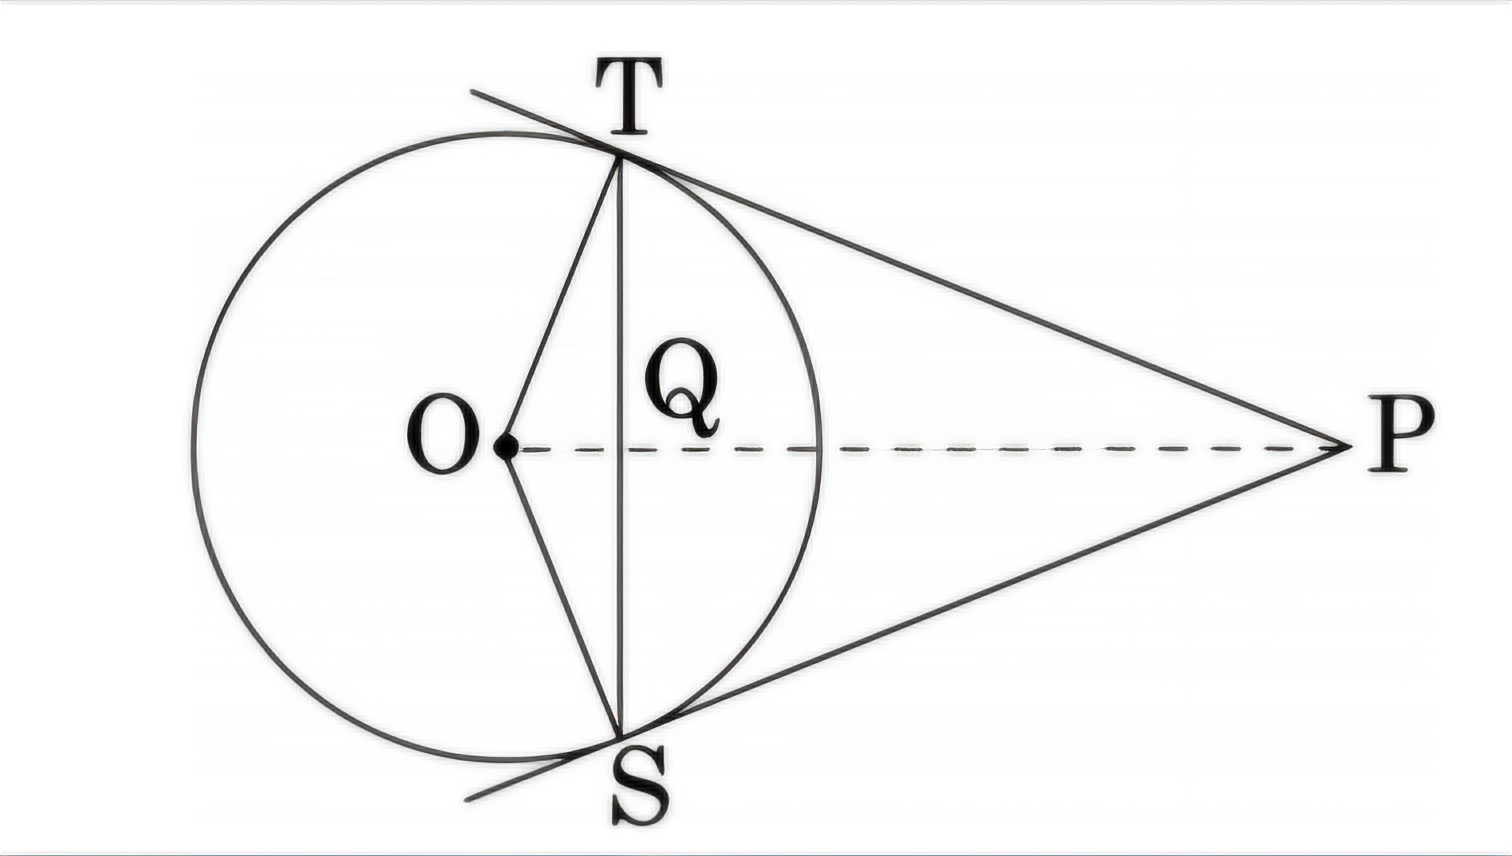
\includegraphics[width=\columnwidth]{./figs/tangentofcircle.jpg}                                                                                        \caption{Two tangents of a circle}                                                                                                                      \label{fig:tangentofcircle}                                                                                                                             \end{figure}                                                                                                                                          
\item Prove that the points $(3, 0), (6, 4)$, and $(-1, 3)$ are the vertices of a right-angled isosceles triangle.
\item A conical vessel, with base radius $5cm$ and height $24cm$, is full of water. This water is emptied into a cylindrical vessel of base radius $10 cm$. Find the height to which the water will rise in the cylindrical vessel. (Use $\pi = \frac{22}{7}$)                                                                                                                                                                                                                                                                                                                                                             
\item In \figref{fig:concentriccircle}, find the area of the shaded region, enclosed between two concentric circles of radii $7cm$ and $14 cm$ where $\angle AOC = 40^{\degree}$. (Use $\frac{22}{7}$)                                                        \begin{figure}[H]                                                                                                                                          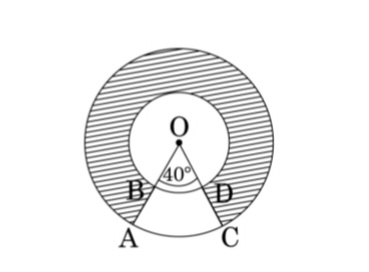
\includegraphics[width=\columnwidth]{./figs/concentriccircle.jpg}
        \caption{Two concentric circles}
	        \label{fig:concentriccircle}                                                                                                                          \end{figure}
\item In \figref{fig:sectorofcircle}, is shown a sector $OAP$ of a circle with center $O$, containing $\angle \theta$. $AB$ is perpendicular to the radius $OA$ and meets $OP$ produced at $B$. Prove that the perimeter of the shaded region is $r\brak{\tan\theta + \sec\theta +\frac{\pi\theta}{180}}$
     \begin{figure}[H]
               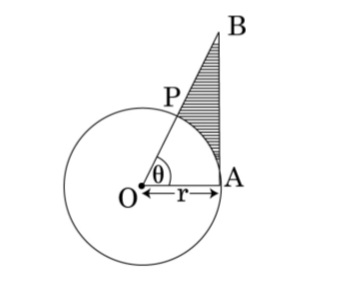
\includegraphics[width=\columnwidth]{./figs/sectorofcircle.jpg}                                                                                      \caption{Sector OAP of a circle}
	                \label{fig:sectorofcircle}
			    \end{figure}   
\item The houses in a row are numbered consecutively from $1$ to $49$. Show that there exists a value of $X$ such that the sum of the numbers of the h    ouses proceeding the house numbered $X$ is equal to sum of the numbers of houses following $X$.      
\item Drawan isosceles $\triangle ABC$, in which $BC = 5.5cm$ and the altitude $AL = 3cm$. Then construct another triangle whose sides are $\frac{3}{4    }$ of the corresponding sides of $\triangle ABC$.                                                                                                      
 \item Prove that the tangent drawn at any point of a circle is perpendicular to the radius through the point of contact.
 \item A rectangular park is to be designed whose breadth is $3 m$ less than its length. Its area is to be $4$ square meters more than the area of a pa    rk that has already been made in the shape of an isosceles triangle with its base as the breadth of the rectangular park and an altitude of $12 m$. Fi    nd the length and breadth of the rectangular park.
\end{enumerate}
  \end{document}
